\section{Simulations} 

Dans cette partie, nous allons nous intéresser à la simulation avec LTSpice des filtres passifs modélisés précédemment via les valeurs des coefficients $g_i$. 

\subsection{Simulation de filtre passe-bas : }

On réalise le montage suivant, on règle la source de tension pour qu’elle ait une amplitude AC d’au moins 1V et on fait une simulation « AC Analysis » de  : 

\begin{figure}[!htbp]
    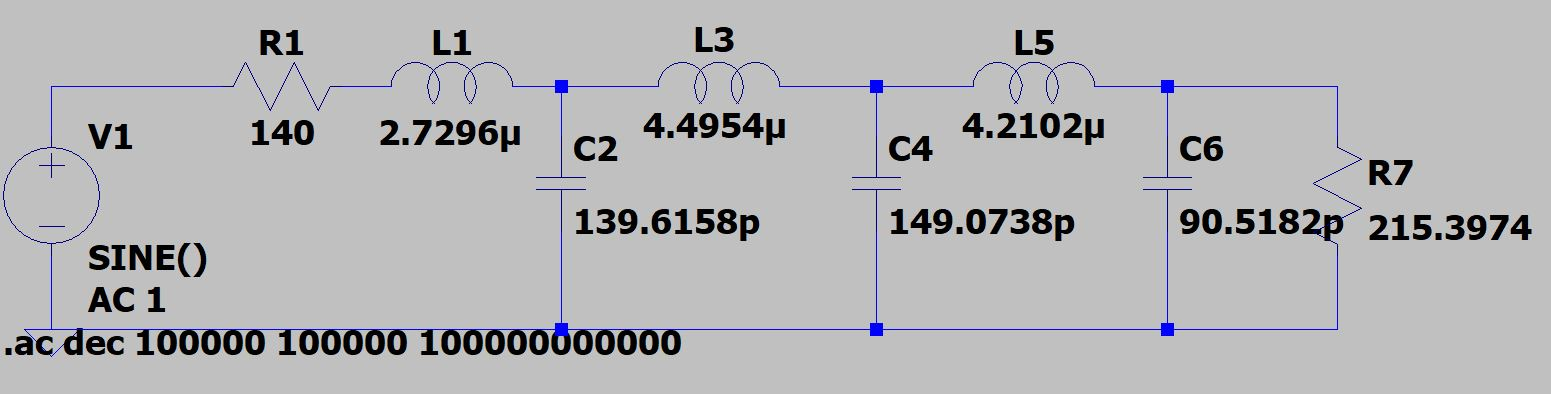
\includegraphics[width=\textwidth,height=\textheight,keepaspectratio]{src/circuits/circuit_passe_basLT.JPG}
    \centering
    \caption{Schéma LTSpice filtre passe-bas Chebyshev d'ordre 6}
\end{figure}
\FloatBarrier

\newpage
La simulation nous donne le diagramme de bode suivant : 

\begin{figure}[!htbp]
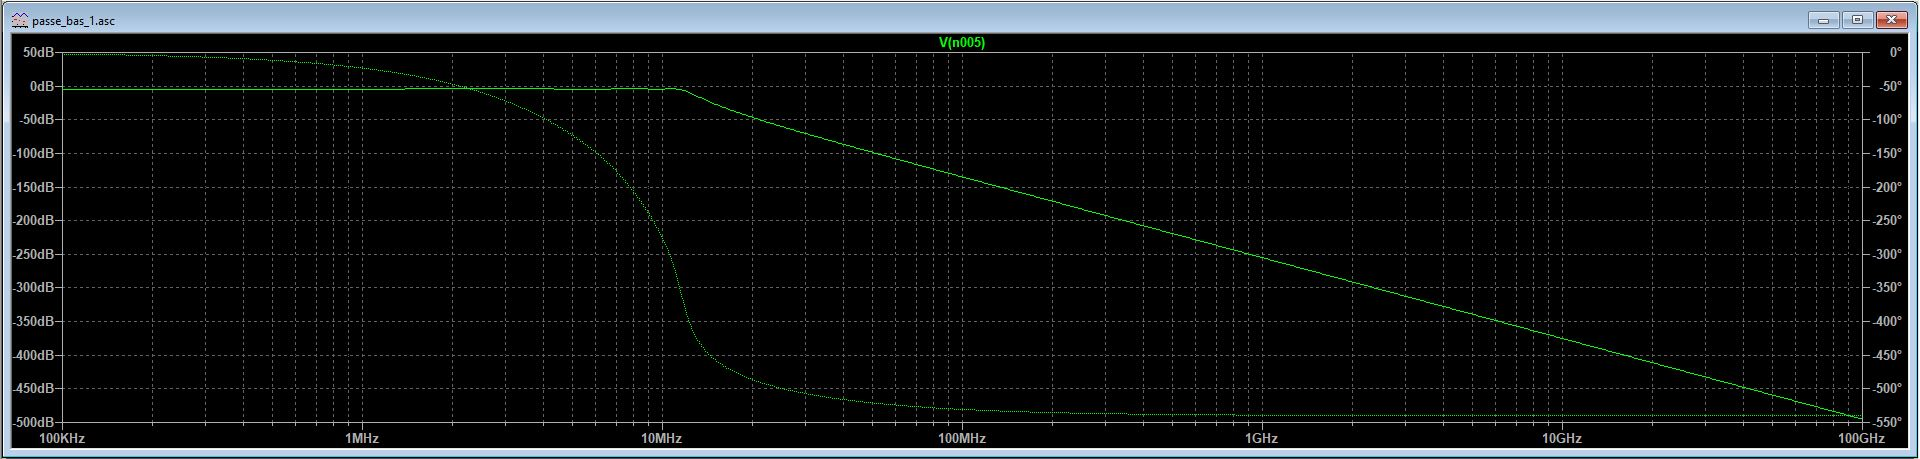
\includegraphics[width=\textwidth,height=\textheight,keepaspectratio]{img_simule/passe_bas_simule.JPG}
    \centering
    \caption{Diagramme de bode LTSpice filtre passe-bas Chebyshev d'ordre 6}
\end{figure}
\FloatBarrier

Nous constatons que : 
\begin{itemize}
  \item Le montage filtre à partir de la fréquence 11.1MHZ 6ième (à 100kHz près) comme indiqué dans le cahier des charges du filtre.
  \item La pente du gain vaut -120dB/dec ce qui correspond à un filtre de 6ième ordre. 
  \item Le déphasage passe de 0° dans la bande passante à -540° lorsque la fréquence tend vers l’infini, ce qui est aussi attendu d’un filtre du 6ième ordre. 
\end{itemize}

\subsection{Simulation de filtre passe-bande :  }

On réalise le montage suivant on applique les mêmes étapes que dans la partie précédente : 

\begin{figure}[!htbp]
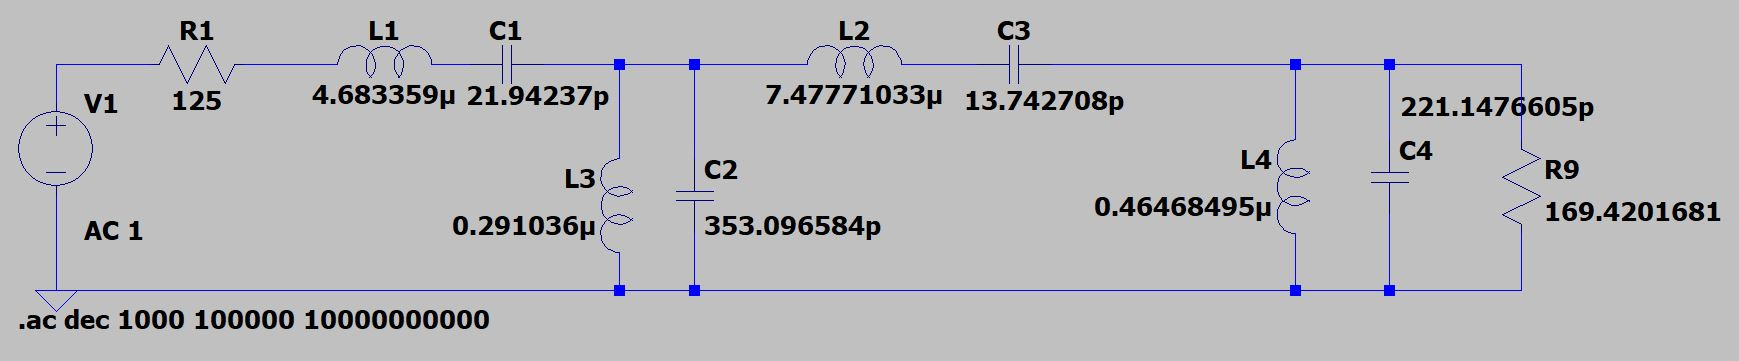
\includegraphics[width=\textwidth,height=\textheight,keepaspectratio]{src/circuits/passe band circuit.JPG}    \centering
    \caption{Schéma LTSpice filtre passe-bande Chebyshev d'ordre 8}
\end{figure}
\FloatBarrier

\begin{figure}[!htbp]
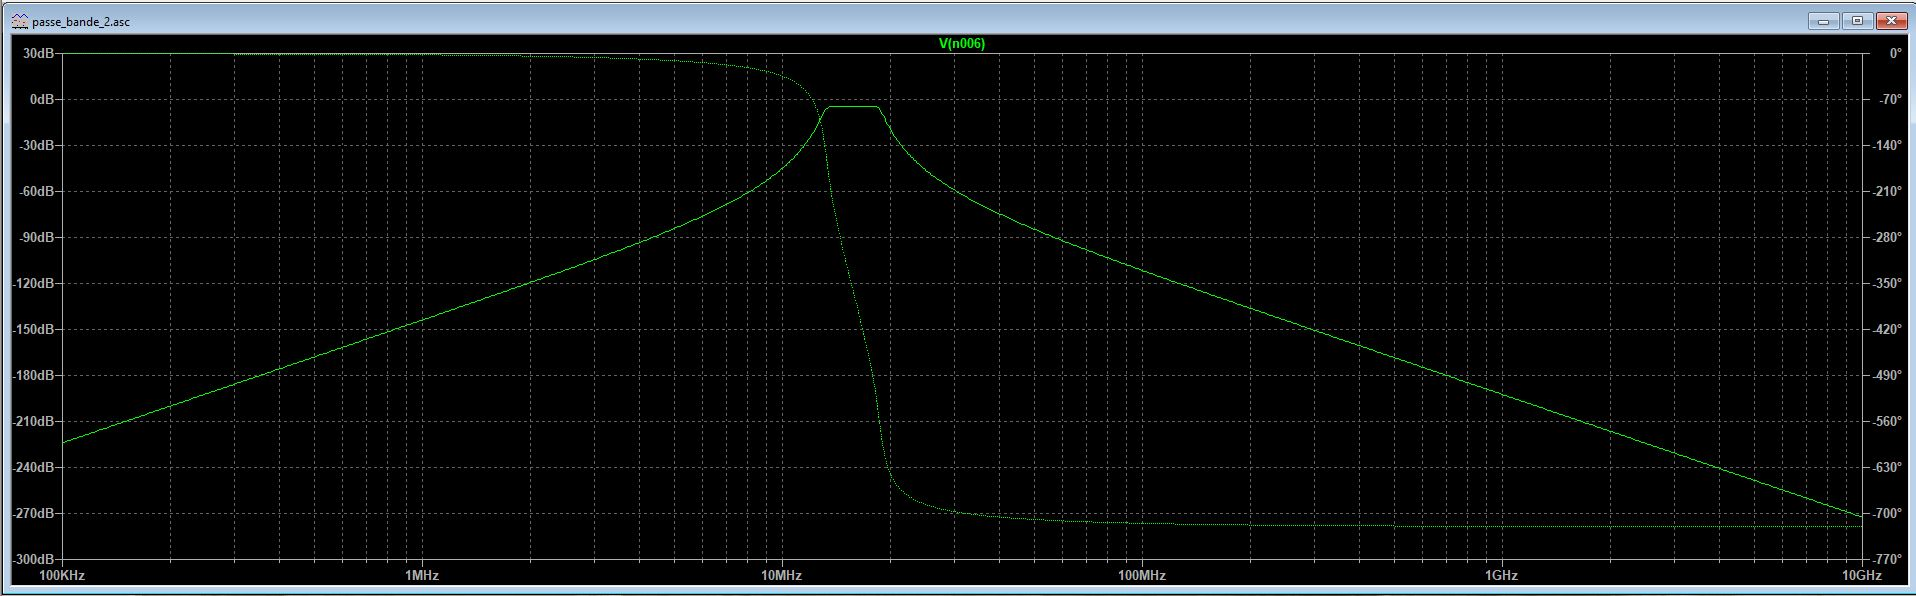
\includegraphics[width=\textwidth,height=\textheight,keepaspectratio]{img_simule/passe_bande_simule.JPG}
\centering
    \caption{Diagramme de bode LTSpice filtre passe-bande Chebyshev d'ordre 8}
\end{figure}
\FloatBarrier

Nous constatons que : 
\begin{itemize}
  \item La bande passante correspond (à 200KHz près, entre 13.345MHz et 18.055MHz) à ce qui est demandé dans le cahier des charges ainsi que la fréquence centrale (15.7MHz à 100KHz près). 
  \item La pente du gain vaut -140dB/dec ce qui correspond à un filtre passe-bande du 8ième ordre. 
  \item Le déphasage passe de 0° à -720°. 
\end{itemize}


\subsection{Simulation de filtre passe-bas elliptique :  }

On réalise ce montage en suivant les mêmes étapes: 

\begin{figure}[!htbp]
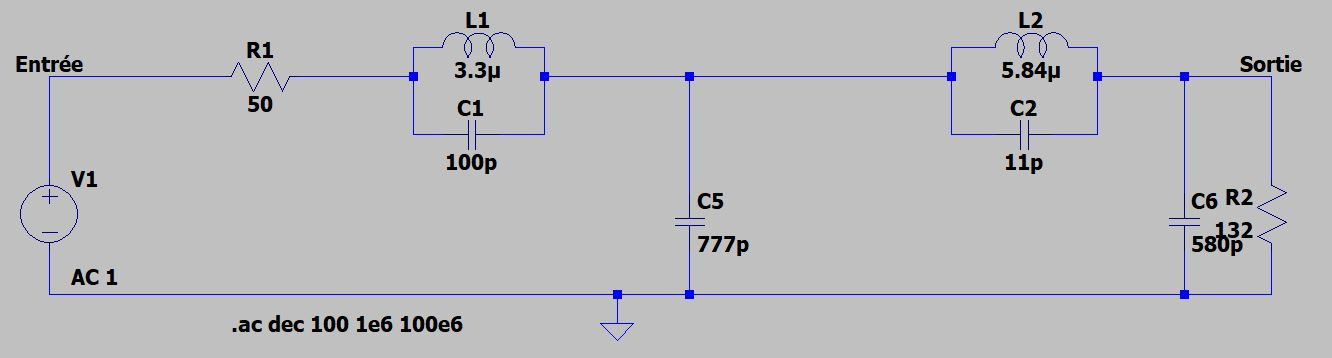
\includegraphics[width=\textwidth,height=\textheight,keepaspectratio]{src/circuits/passe bas elliptique.JPG}
\centering
    \caption{Schéma LTSpice filtre passe-bas Elliptique d'ordre 4}
\end{figure}
\FloatBarrier

\begin{figure}[!htbp]
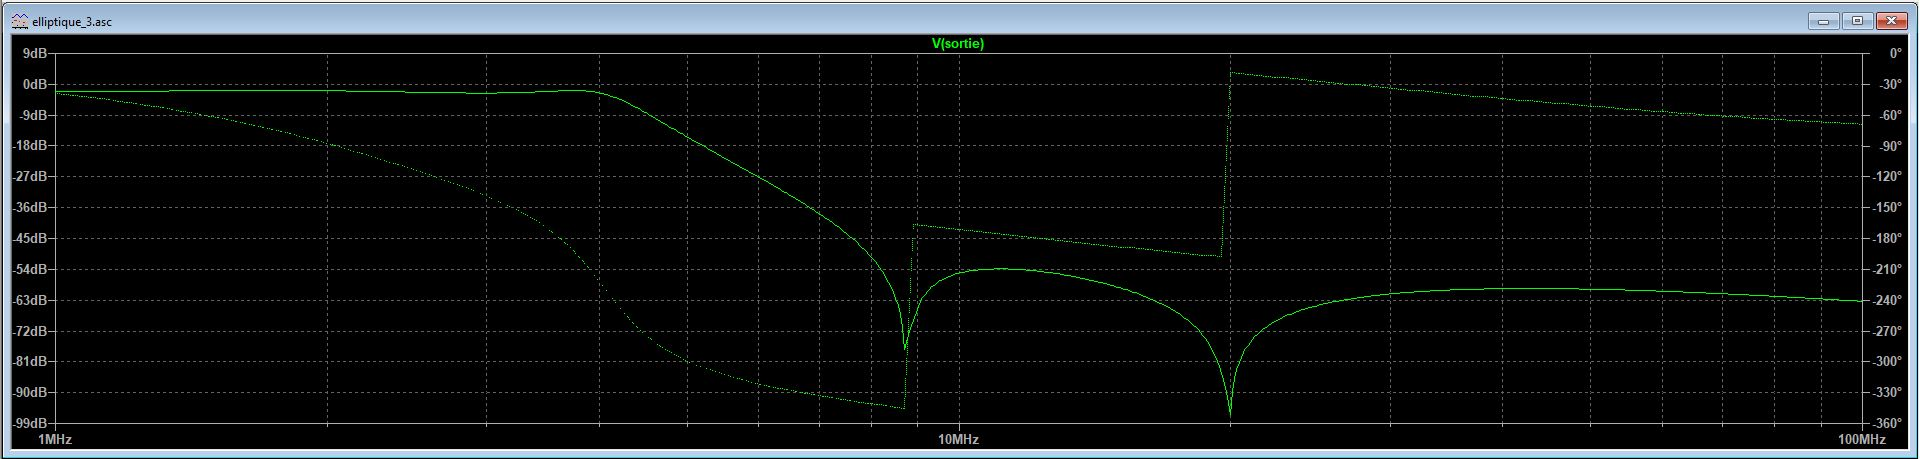
\includegraphics[width=\textwidth,height=\textheight,keepaspectratio]{img_simule/elliptique_simule.JPG}
\centering
    \caption{Diagramme  de bode LTSpice filtre passe-bas Elliptique d'ordre 4}
\end{figure}
\FloatBarrier

Nous constatons que : 

\begin{itemize}
  \item La fréquence de coupure vaut à peu près 4.1MHz ce qui correspond à la valeur du cahier des charges. 
  \item L’ondulation dans la bande coupée à 10MHz vaut -54db/dec (-52dB/dec dans le cahier des charges). 
\end{itemize}


Donc les diagrammes de Bode du montage simulé respectent les critères caractéristiques (fréquence de coupure, bande passante, déphasage et pente) aux gabarits des montages théoriques réalisés via les coefficients $g_i$, cependant, il existe de légères différences sur l’atténuation maximale dans la bande passante pour le filtre passe bas elliptique (de -1dB à -2dB) et une différence remarquable pour les filtres passe-bas et bande type Chebyshev (de -0.1dB et -0.2dB respectivement à -4dB environ pour les deux).